\chapter{Experiments and results}

\label{ch:Experiments and results}

\setlength{\parindent}{4em}
\setlength{\parskip}{1em}
\renewcommand{\baselinestretch}{1.5}

\section{Hardware for the experiment}

\hspace{1.5cm} In our project, first, we plan how to investigate the EEG data from the subject. There are 2 categories to investigate the data those are software and hardware. When we know like that we go to study how is it different between software and hardware that use in this project and when we already study in it, so we know that hardware is better than software ????? and we choose it and We plan to design the hardware to use it in the experiment. This is materials that we use in our project.

\subsection{EPOC headset by Emotiv\texttrademark}
\hspace{1.5cm} The wireless headset Emotiv EPOC research edition, it records EEG data in 14 channel of International 10-20 Locations system with Sequential sampling rate at 128 per second (2048 Hz internal) with resolution 14 bit (16 bit Analog to digital converter, 2-bit instrumental noise floor discarded), the bandwidth is in range 0.2 to 45 Hz with digital notch filters at 50Hz and 60 Hz.

We use this equipment in our experiment to obtain the EEG from the subjects and we use EEG that we can obtain from the user to apply in our project.
\begin{figure}[ht]
	\centering
	\includegraphics[scale = 0.09]{chapter3/36.pdf}
	\caption{EPOC headset by Emotiv\texttrademark}
\end{figure}

\subsection{Arduino Uno}
\hspace{1.5cm} The Arduino Uno is a microcontroller board based on the ATmega328 that is an open source platform. It has 14 input/output pins6 analog inputs, a 16 MHz quartz crystal, a USB connection, a power jack, an ICSP header and a reset button, The USB connection for upload the software into the Arduino and VCC or supply for connecting the peripheral circuit.

In our experiment, we use the Arduino UNO board to control the hardware which we use to stimuli subjects to get the EEG from subjects to apply it in our project.
\begin{figure}[ht]
	\centering
	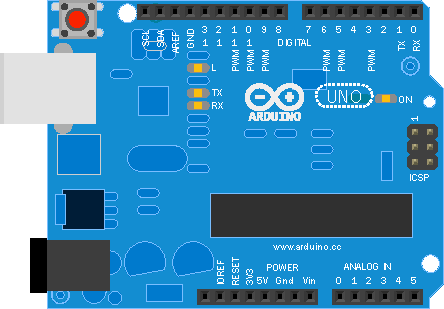
\includegraphics[scale = 0.8]{chapter3/38.pdf}
	\caption{Illustrate of Arduino UNO board}
\end{figure}

\subsection{Gravitech Gerora WS2812S LED}
\hspace{1.5cm} The full-color Light-emitting diode (LED) driver which is use for stimulating the subject has an LED light WS2812 model mounted on. It can chain connected with the same model. It can be controlled by a programmed Arduino. The luminous intensity is 550 to 700 mega candela for red, 1100-1400 mcd for green, and 200-400 mcd for blue.

For this hardware, we use it be flickers to blink the LED that in this board. We can control the frequency, intensity, and color of LED. This hardware is controlled by the Arduino Uno board to stimuli subjects to get the EEG to apply in our project.
\begin{figure}[ht]
	\centering
	\includegraphics[scale = 0.4]{chapter3/37.pdf}
	\caption{Gravitech Gerora LED base on WS2812}
\end{figure}

\subsection{Visual stimulus (ERP)}
\hspace{1.5cm} As the Figure \ref{fig:vs} show our prototype visual stimulator. It consists of the Arduino board and gravitech gerora WS2812 LED board. This stimulator uses to stimuli subjects to get EEG. This stimulator blinks the light from LED 1 to LED 4 respectively. This stimulator was used in Experiment I and II.

\begin{figure}[ht]
	\centering
	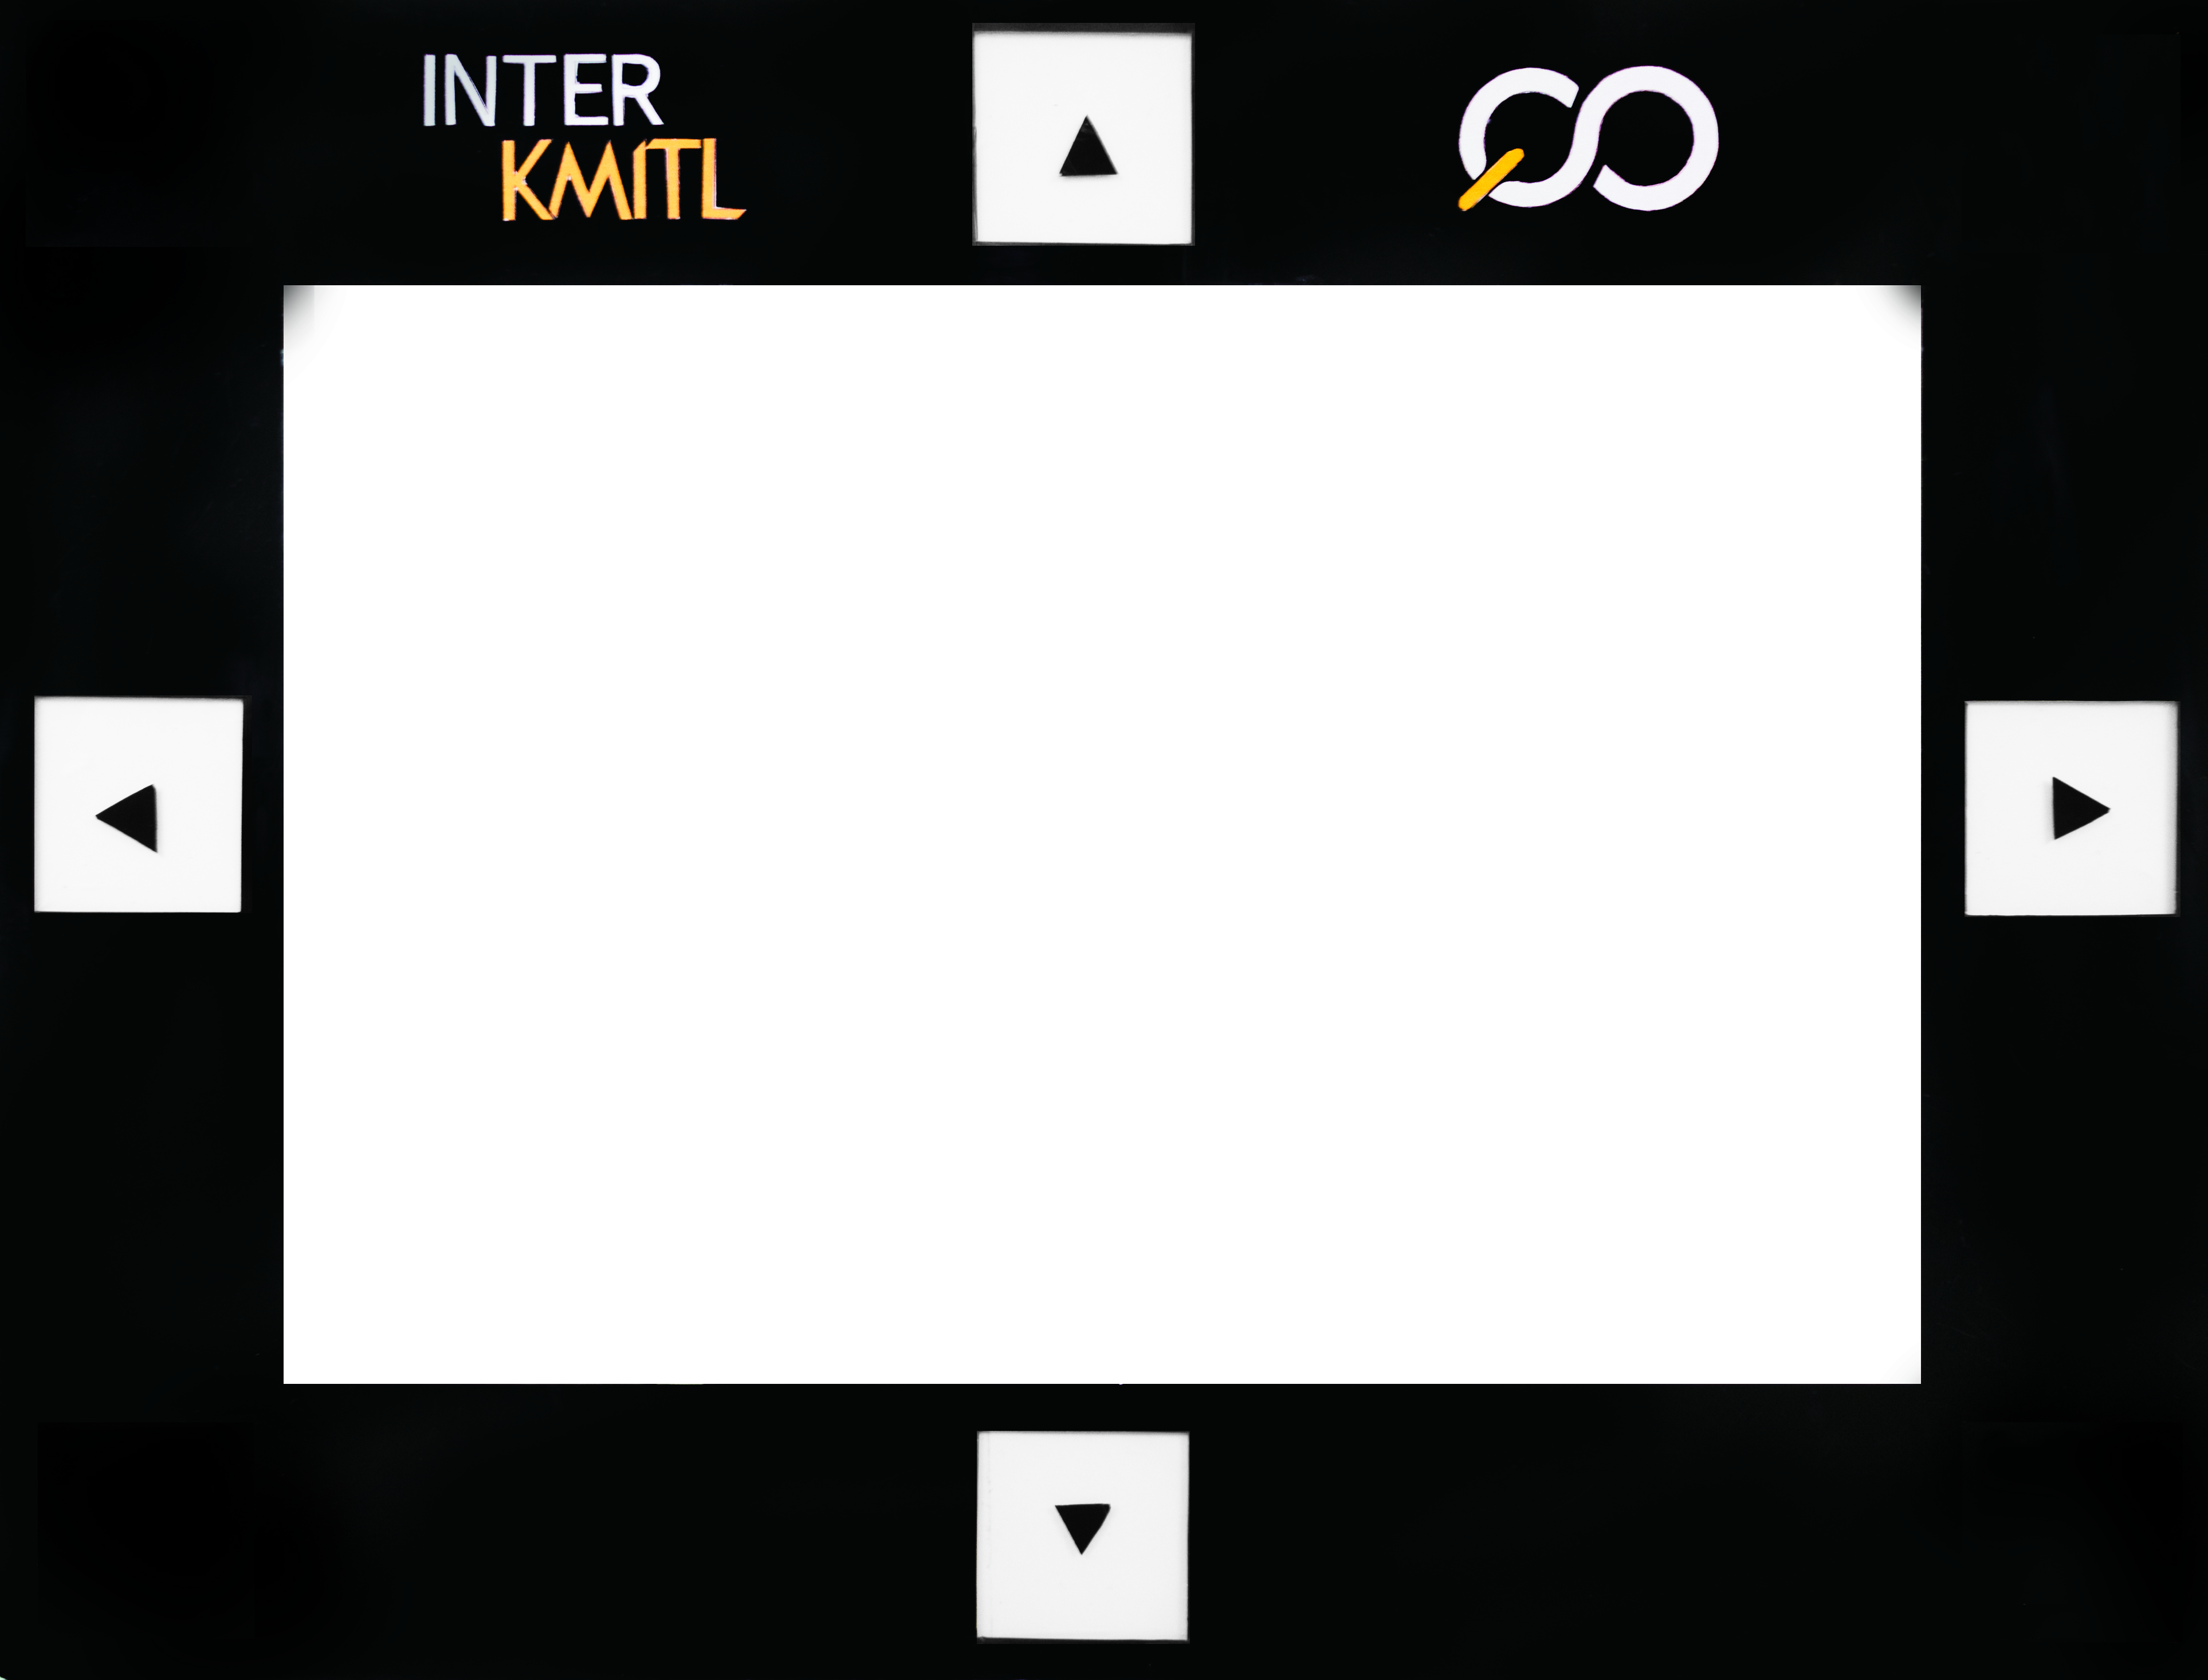
\includegraphics[scale=0.25]{chapter7/frame_4.jpg}
	\caption{Visual Stimulator with four targets used for ERPs}
	\label{fig:vs}
\end{figure}

\newpage
\subsection{Visual stimulus (SSVEP)}
\hspace{1.5cm} This visual stimulator was developed based on the previous visual stimulus(ERP). The difference between this stimulator and previous stimulator is this stimulator has 8 flickers and each flicker has different frequencies, which was used in Experiment III and IV.

\begin{figure}[ht]
	\centering
	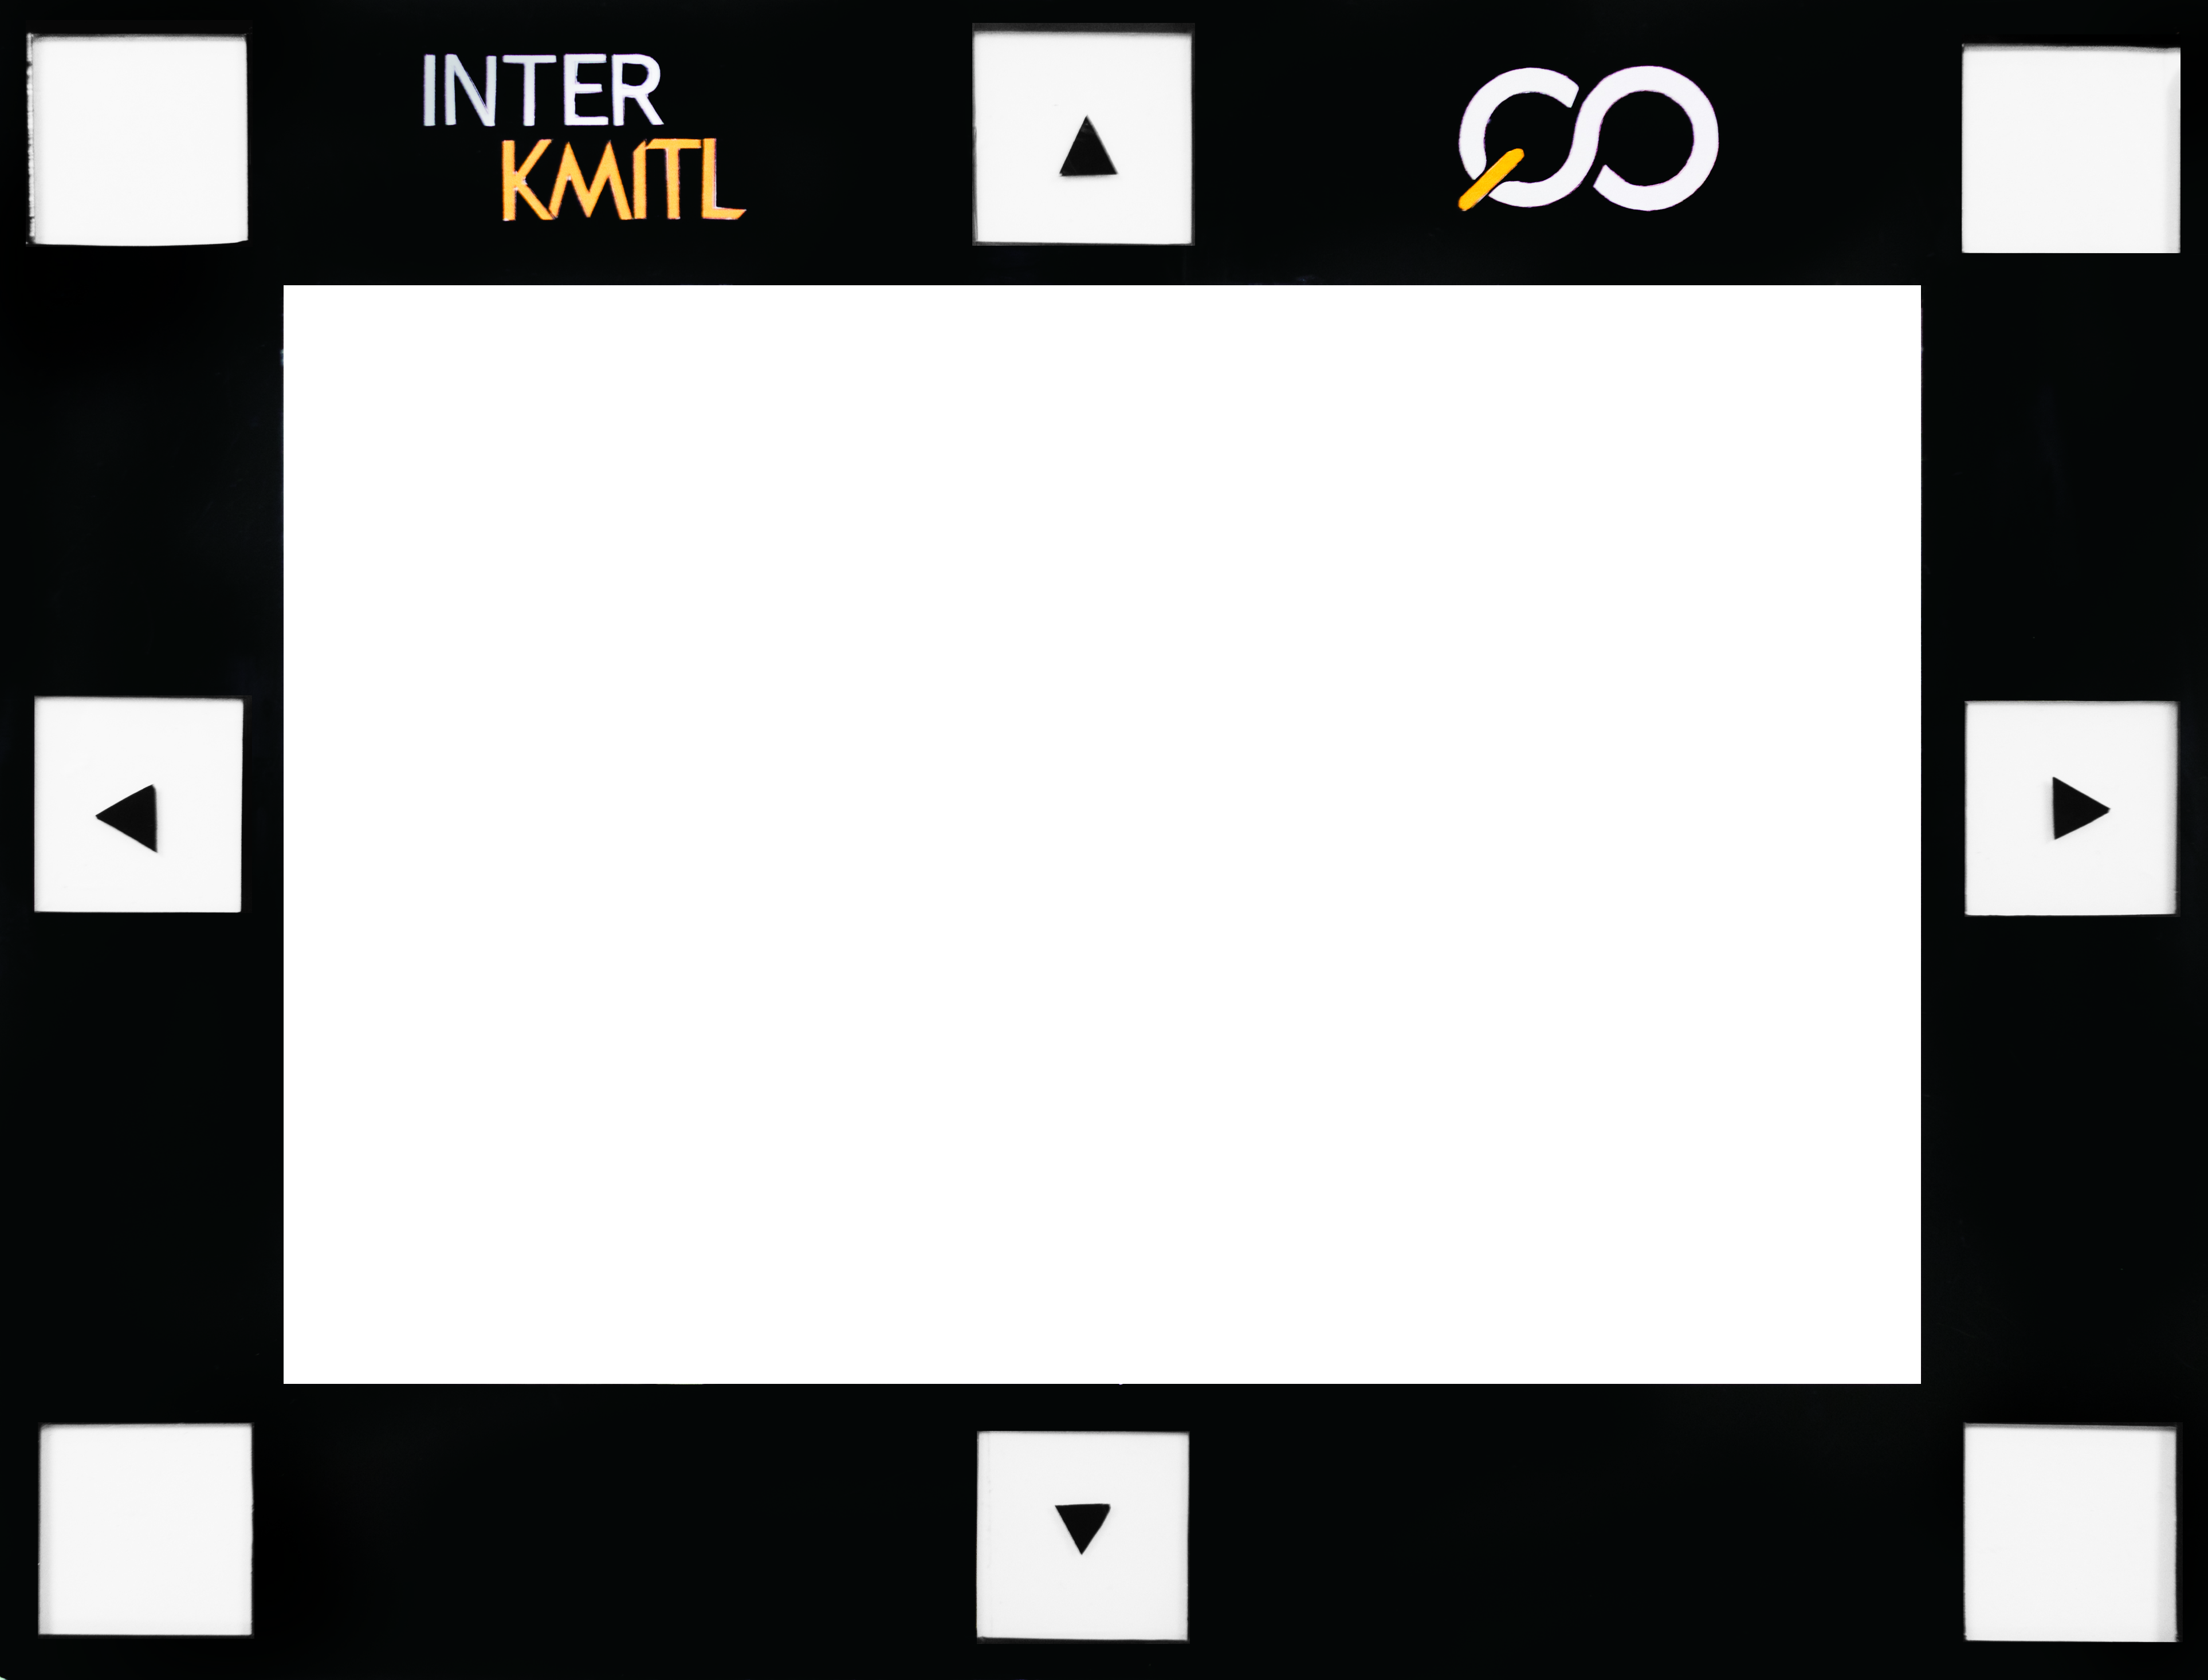
\includegraphics[scale=0.25]{chapter7/frame_8.jpg}
	\caption{Visual Stimulator with eight targets used for SSVEP}
\end{figure}

\newpage
\section{Experiment I}
\subsection{Experimental Paradigm I}
\begin{itemize}
\item{\textbf{Subjects}}\newline
In this experiment, we use 4 subjects. There are SS,OK,WP and NT that is the nickname and firstname of subjects.

\newcolumntype{P}[1]{>{\centering\arraybackslash}p{#1}}
\begin{table}[ht]
\centering
\begin{tabular}{| P{.2\linewidth} | P{.2\linewidth} | P{.2\linewidth} |}
			\hline 
			\textbf{Subjects} & \textbf{Age}  & \textbf{Sex}\\
			\hline 
			SS & 22 & Male\\
			\hline 
			OK & 22 & Male\\
			\hline 
			WP & 21 & Male\\
			\hline 
			NT & 21 & Male\\
			\hline
		\end{tabular}       
\caption{Subjects of experiment I}
\label{table:subject}
\end{table}

\item{\textbf{Visual Stimulator}}
In this experiment, we use 4 visual stimulator[LED 1($Y_1$),LED 2($Y_3$),LED 3($Y_5$),LED 4($Y_7$)]
\item{\textbf{Stimulus}}
For one trial, we use 11, 15, 19, 23 seconds respectively.
\item{\textbf{Trials}}
We recorded 3, 5, 7, 9 times for each set of parameter.
\item{\textbf{Environment}}
In this experiment, we control the light illuminate value at 37 Lux.
	\item{\textbf{Parameters}}\\
There are 4 parameters. First is flickering type, stimulus, sample length and epoch time.
\end{itemize}

\newcolumntype{P}[1]{>{\centering\arraybackslash}p{#1}}
\begin{table}[ht]
\centering
\begin{tabular}{| P{.3\linewidth} | P{.3\linewidth} | P{.3\linewidth} |}
			
			\hline 
			\textbf{Parameter} & \textbf{Experiment A}  & \textbf{Experiment B}\\
			\hline 
            Stimulus & static & Modular   \\
			\hline 
            Flickering type & \multicolumn{2}{c}{Regualr} \vline\\
			\hline 
			Sample Length & \multicolumn{2}{c}{64samples/epoch} \vline\\
			\hline 
			Epoch time & \multicolumn{2}{c}{500 ms} \vline\\
			\hline
		\end{tabular}       
\caption{Experimental paradigm I}
\label{table:stimulus}
\end{table}

In this experiment, we set the duty-cycle to be 0.7 and light intensity to be 50\%. The experimental paradigm is shown in Table 7.2, we set the flickering type, sample length, epoch time, duty cycle, intensity and frequency to be the same. There is some difference in stimulus. We have 2 experiment of stimulus. First is regular, static means a flicker will blink 1 time per LED is shown in Figure 7.6. Modular means a flicker will blink 3 times for each LED as shown in Figure 7.7. We will do this for 3, 5, 7 and 9 trials respectively for each subject to obtain the EEG. We obtain the data around 20 times for each subject and calculate average from data to obtain the accuracy of this experiment.

\begin{figure}[ht]
	\centering
	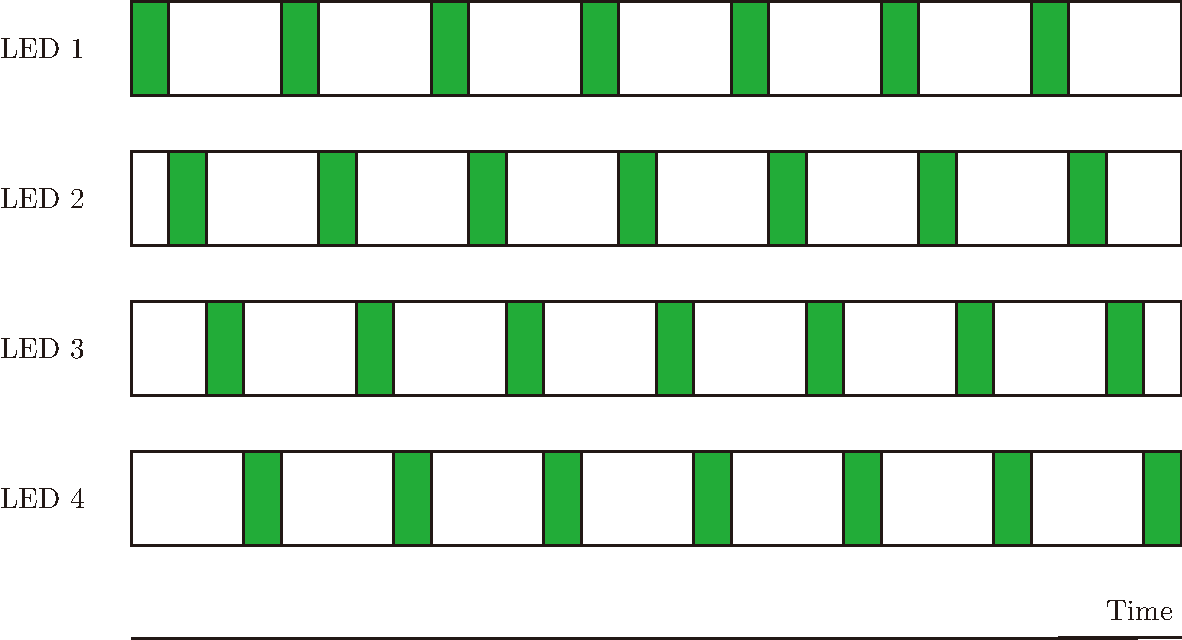
\includegraphics[scale = 0.65]{chapter7/sta_nor.pdf}
	\caption{Stimulus : Regular}
\end{figure}

\begin{figure}[ht]
	\centering
	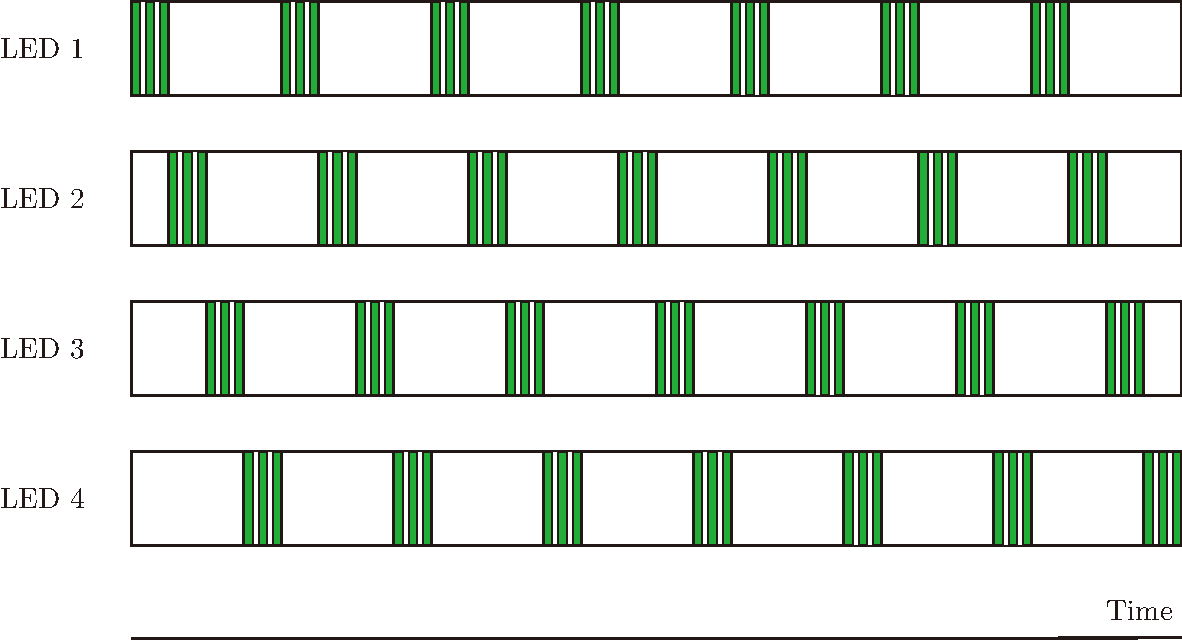
\includegraphics[scale = 0.65]{chapter7/mod_nor.pdf}
	\caption{Stimulus : Modular}
\end{figure}

\newpage
\subsection{Experiment result I}

\begin{figure}[ht]
	\centering
	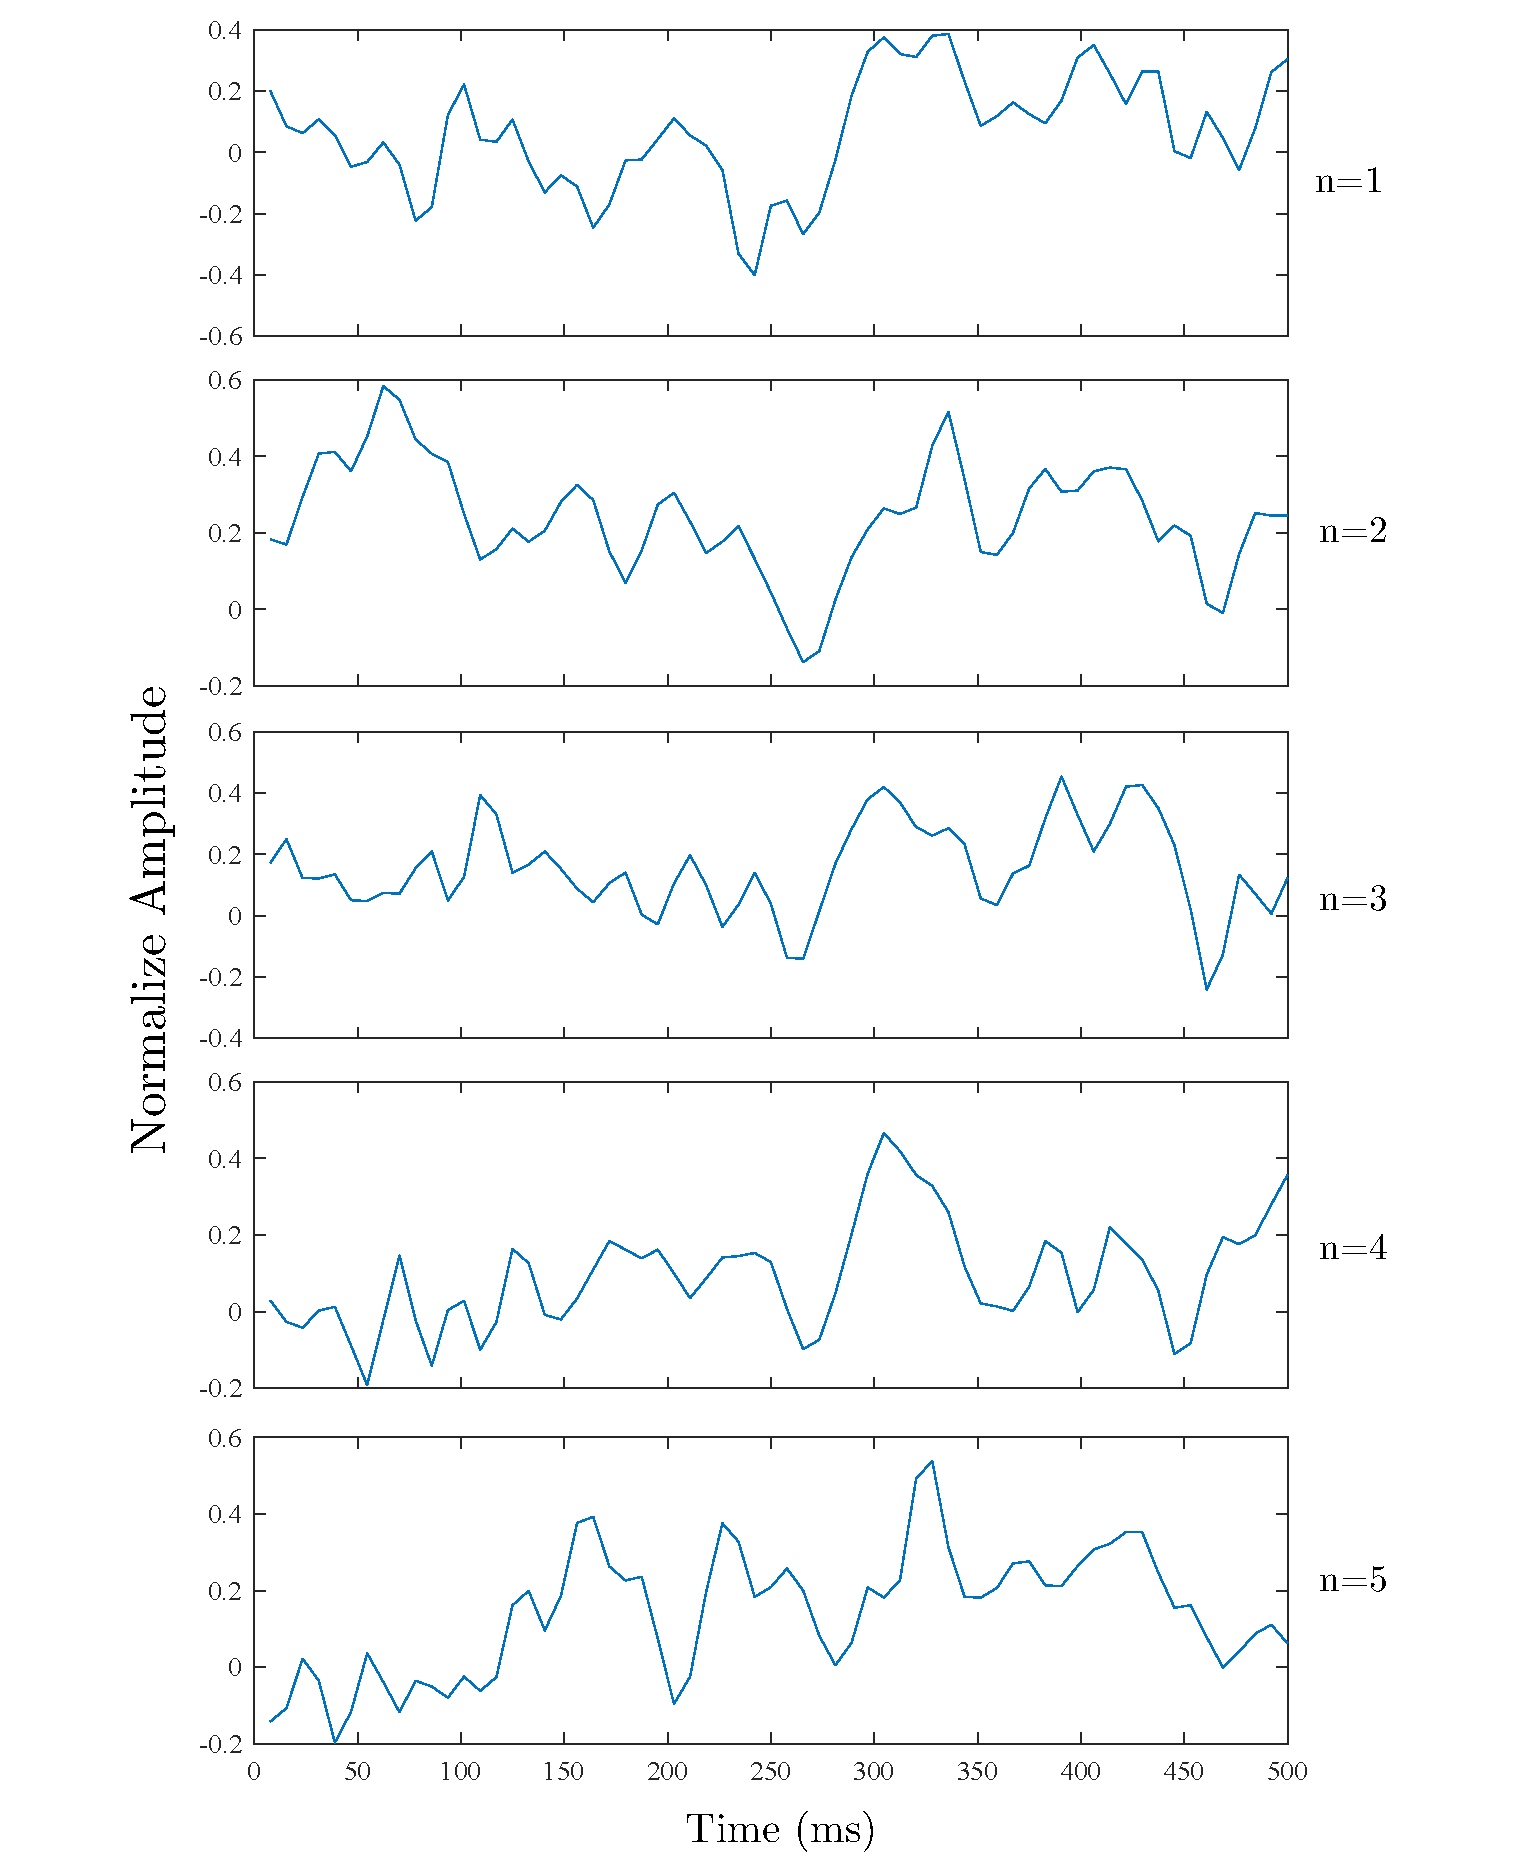
\includegraphics[scale = 0.4]{chapter7/rawdata.pdf}
	\caption{Raw data of EEG from subject "OK", n trials ; n = number of trials for each subjects to calculate the averages.}
		\label{fig:raw_data}
\end{figure}

\begin{figure}[ht]
	\centering
	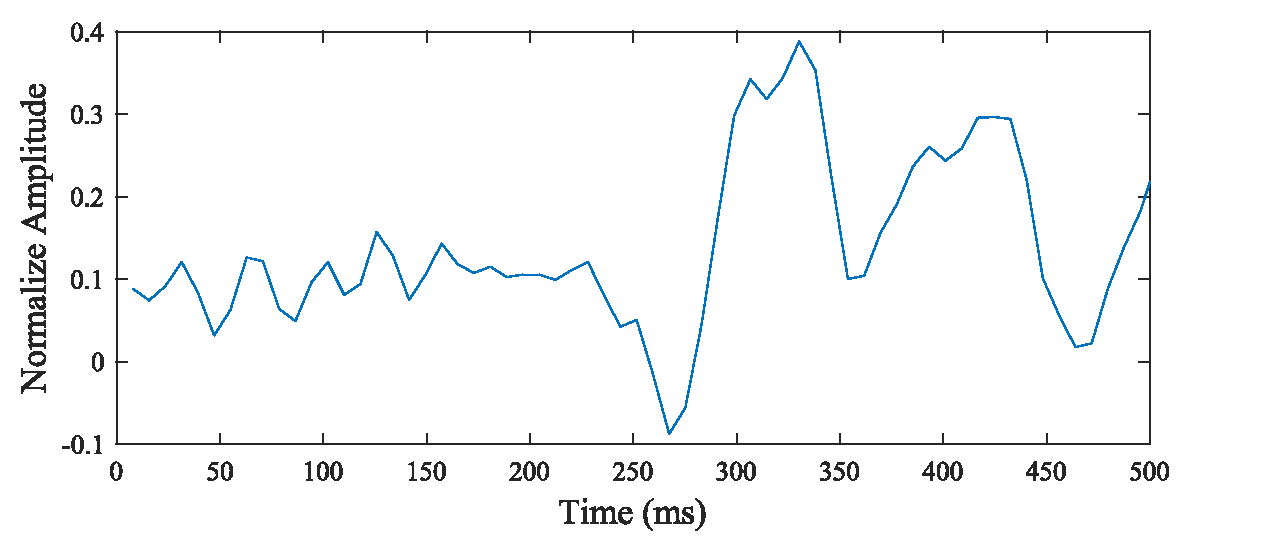
\includegraphics[scale = 0.4]{chapter7/rawavg.pdf}
	\caption{The averaged EEG data of subject "OK" from raw data in Figure 7.8 }
		\label{fig:avg}
\end{figure}

From the Figure \ref{fig:raw_data}, displays an example of raw EEG data obtained from the  subject "OK". 'n' in Figure \ref{fig:raw_data} means the number of trials for each subject .In this figure, we adjust n to 5. After obtaining these 5 trials of raw data, we will calculate the average of these raw data as shown in Figure \ref{fig:yx}


\begin{figure}[ht]
	\centering
	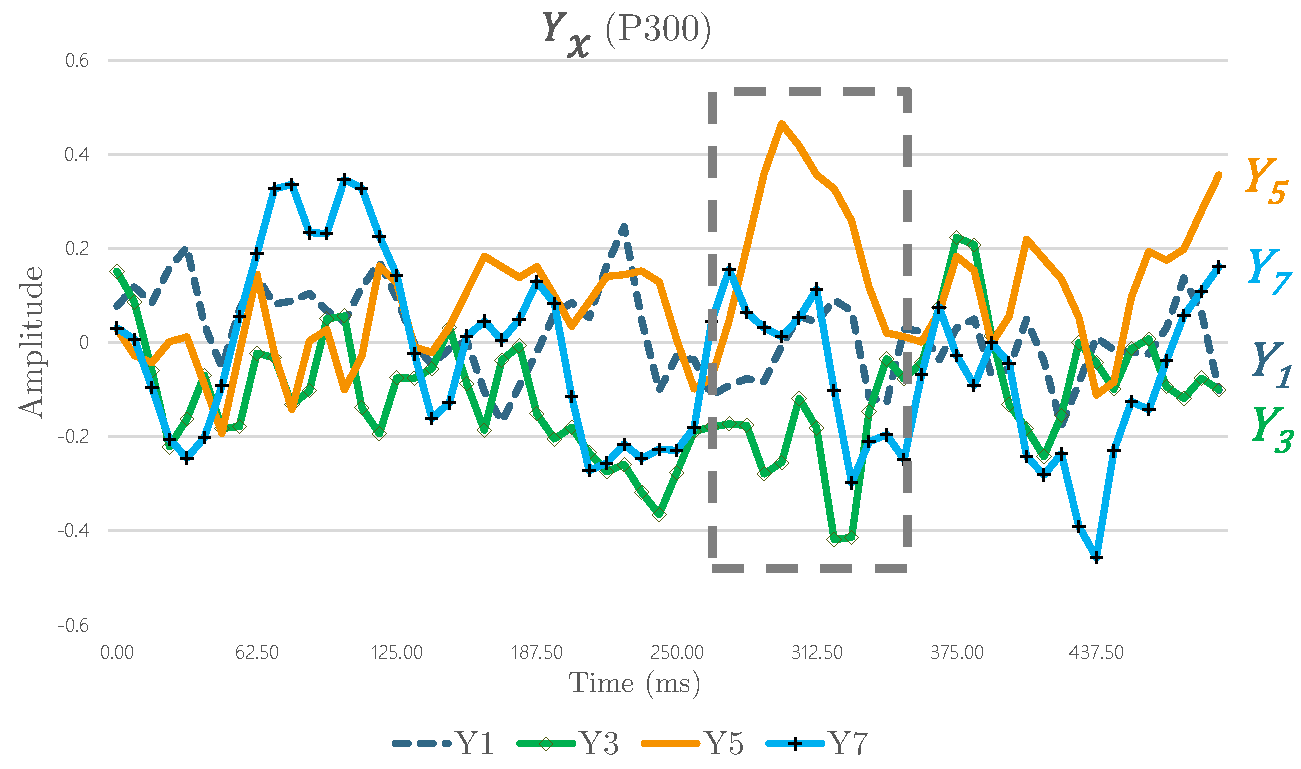
\includegraphics[width=\textwidth]{chapter7/erp_result.pdf}
	\caption{EEG data of subject "OK" ,trial = 5 from flickers $Y_1,Y_3,Y_5$ and $Y_7$ }
		\label{fig:yx}
\end{figure}

From the figure \ref{fig:avg}, we obtain the average of EEG data from subject "OK" ,which uses only in 1 flicker. However, we use 4 flickers in our experiment. When we merge all of average EEG data, we will get the data in figure \ref{fig:yx}. In the figure \ref{fig:yx}, we obtain the EEG data of flickers line $Y_1,Y_3,Y_5$ and $Y_7$ for experiment I from trial= 5, subject = "OK". When we receive the EEG data of each flicker (Figure \ref{fig:yx}), we use a range of 290-350 millisecond to classify which flicker that the subject fixate. From figure \ref{fig:yx}, we will see the 4 lines of the graph. $Y_1$ the EEG data from flicker 1, $Y_3$ is from flicker 2, $Y_5$ is from flicker3, and $Y_7$ is from flicker 4. Each line means that we collect the data of the subject for 3 trials and compute the average of the EEG data that we get in each line. When we have already computed the average, we apply the normalization to all of the data which are averages to compare with each other. In this figure, the flicker that the subject fixate is $Y_5$ or flicker 3.

\begin{figure}[ht]
	\centering
	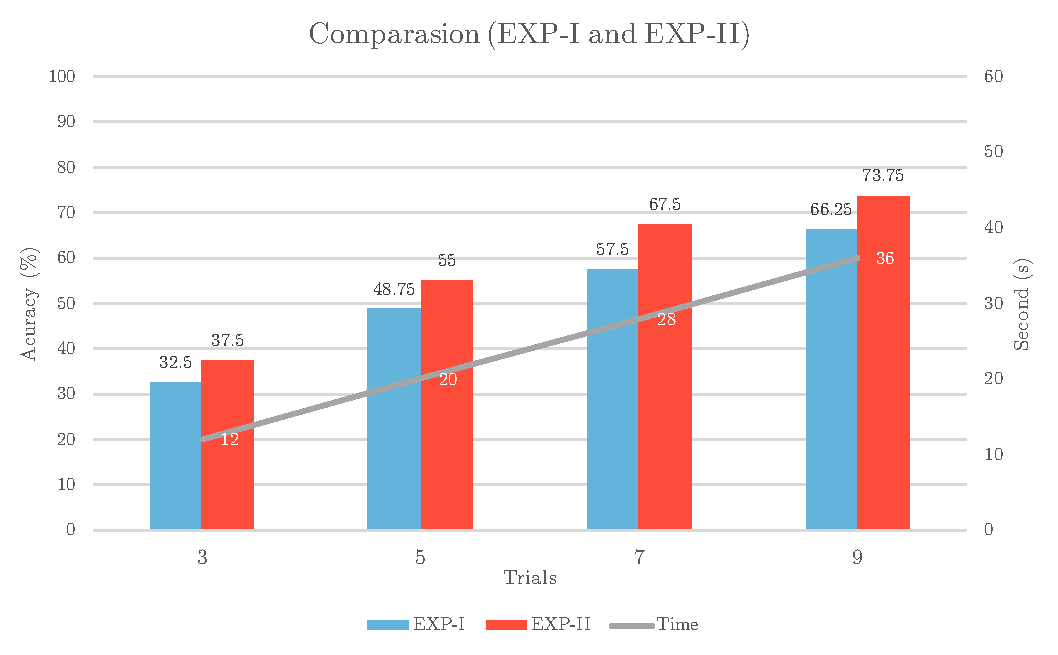
\includegraphics[scale = 0.8]{chapter7/result1_2.pdf}
	\caption{Comparison between the result of experiment A and B}
	\label{fig:compare1}
\end{figure}

From the figure \ref{fig:compare1}, we have a comparison graph of the first experiment A and the second experiment B. Both are different in stimulus. EXP A's stimulus is static, whereas EXP B has a modular stimulus. This graph illustrates the accuracy of EXP A and EXP B, where the trial = 7. The accuracy of EXP A is equal to 57.5\% and EXP B is equal to 67.5\%. We can see that EXP B is more accurate than EXP A in any trials that we use.


\begin{table}[ht]
\centering
\begin{tabular}{| c | c | c | c | c |}

			\hline 
			\multirow{2}{*}{\textbf{Trial}} & 
  			\multirow{2}{*}{\textbf{Total time [s]}}  & 
            \multirow{2}{*}{\textbf{Subject}} &
            \multicolumn{2}{c|}{\textbf{Accuracy of stimulus}} \\
            \cline{4-5}
            &&&\multicolumn{1}{c|}{\textbf{Regular}} &\multicolumn{1}{c|}{\textbf{Modular}}  \\
			\hline 
			\multirow{4}{*}{3}&\multirow{4}{*}{11}&OK&25&40 \\
			\cline{3-5}
			&&WP&40&40 \\ \cline{3-5}
			&&SS&35&30 \\ \cline{3-5}
			&&NT&30&40 \\
            \hline
			\multirow{4}{*}{5}&\multirow{4}{*}{15}&OK&45&45 \\
			\cline{3-5}
			&&WP&50&55 \\ \cline{3-5}
			&&SS&45&65 \\ \cline{3-5}
			&&NT&55&55 \\
            \hline
            \multirow{4}{*}{7}&\multirow{4}{*}{19}&OK&60&65 \\
			\cline{3-5}
			&&WP&55&70 \\ \cline{3-5}
			&&SS&55&70 \\ \cline{3-5}
			&&NT&60&65 \\
            \hline 
            \multirow{4}{*}{9}&\multirow{4}{*}{23}&OK&65&70 \\
			\cline{3-5}
			&&WP&65&80 \\ \cline{3-5}
			&&SS&70&75 \\ \cline{3-5}
			&&NT&65&70 \\
            \hline 
		\end{tabular}       
\caption{Experiment result I}
\label{table:result1}
\end{table}

The result of this experiment is shown in Table \ref{table:result1} with the same set of parameter for each stimulus, sample length, epoch time, duty cycle, intensity, and frequency. From the Table \ref{table:stimulus},the first row, we can see the accuracy of "SS" in modular is better than static in the same row. Another subject "WP" in the fourteenth row, we can see the accuracy of modular is better than static too. We found each subject have better accuracy in the modular than static of stimulus. We found another thing that is the trial of the experiment. We will compare the accuracy between "OK" in the first row and "OK" in fourteenth row. The result is "OK" in the fourteenth row is better than "OK" in the first row. The main factor is the number of trial that we use in each experiment. We found that when we use more trials, the accuracy is increased too.

\newpage
\section{Experiment II}
\subsection{Experimental Paradigm II}
\begin{itemize}
\item{\textbf{Subjects}}\newline
In this experiment, we use 4 subjects. There are SS,OK,WP and NT that is the nickname and firstname of subjects.


\begin{table}[ht]
\centering
\begin{tabular}{| P{.2\linewidth} | P{.2\linewidth} | P{.2\linewidth} |}
			\hline 
			\textbf{Subjects} & \textbf{Age}  & \textbf{Sex}\\
			\hline 
			SS & 22 & Male\\
			\hline 
			OK & 22 & Male\\
			\hline 
			WP & 21 & Male\\
			\hline 
			NT & 21 & Male\\
			\hline
		\end{tabular}       
\caption{Subjects of experiment II}
\label{table:2}
\end{table}

\item{\textbf{Visual Stimulator}}
In this experiment, we use 4 visual stimulator[LED 1($Y_1$),LED 2($Y_3$),LED 3($Y_5$),LED 4($Y_7$)]
\item{\textbf{Stimulus}}
For one trial, we use 11, 15, 19, 23 seconds respectively.
\item{\textbf{Trials}}
We recorded 3, 5, 7, 9 times for each set of parameter.
\item{\textbf{Environment}}
In this experiment, we control the light illuminate value at 37 Lux.
	\item{\textbf{Parameters}}\\
There are 4 parameters. First is flickering type, stimulus, sample length and epoch time.
\end{itemize}


\begin{table}[ht]
\centering
\begin{tabular}{| P{.3\linewidth} | P{.3\linewidth} | P{.3\linewidth} |}
			
			\hline 
			\textbf{Parameter} & \textbf{Experiment A}  & \textbf{Experiment B}\\
			\hline 
			Flickering type & Regular & Uniform random   \\
			\hline 
			Stimulus & \multicolumn{2}{c}{Modular} \vline\\
			\hline 
			Sample Length & \multicolumn{2}{c}{64samples/epoch} \vline\\
			\hline 
			Epoch time & \multicolumn{2}{c}{500 ms} \vline\\
			\hline
		\end{tabular}       
\caption{Experimental paradigm II}
\label{table:paradigm2}
\end{table}

In this experiment, we set it to be the same as experiment I. However, there is a difference in flickering type. In this experiment, we use a regular, and uniform random flickering types. The regular flickering type means that the flicker will blink from LED1 to LED4 respectively. The uniform random flickering type is used to randomly select the flickers to blink. We have 3,5,7 and 9 trials for each subject to obtain the EEG to be the same as experiment I. We will obtain the EEG and calculate the average and accuracy of this experiment.

From the result of experiment I, the modular stimulus is better than static stimulus. So, we will use the modular stimulus in this experiment. In this experiment, the flickers will be the same as figure\ref{fig:mod_reg} and figure \ref{fig:mod_uni}.
In figure \ref{fig:mod_reg} is shown the regular flickering type with the modular stimulus. The flicker will blink from LED1 to LED4 and it will blink 3 times per each LED. In the same way, the figure \ref{fig:mod_uni} is shown the uniform random flickering type with the modular stimulus that means each flicker will blink randomly and blink 3 time for each flicker.

\begin{figure}[ht]
	\centering
	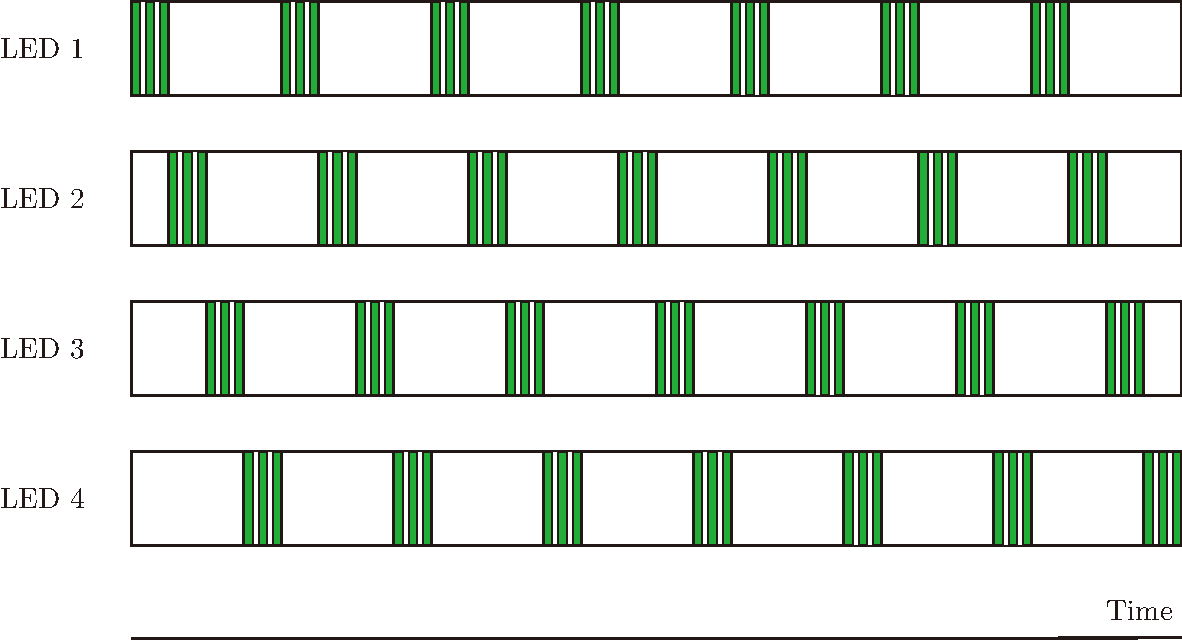
\includegraphics[scale = 0.65]{chapter7/mod_nor.pdf}
	\caption{Flickering type : Regular}
    \label{fig:mod_reg}
\end{figure}

\begin{figure}[ht]
	\centering
	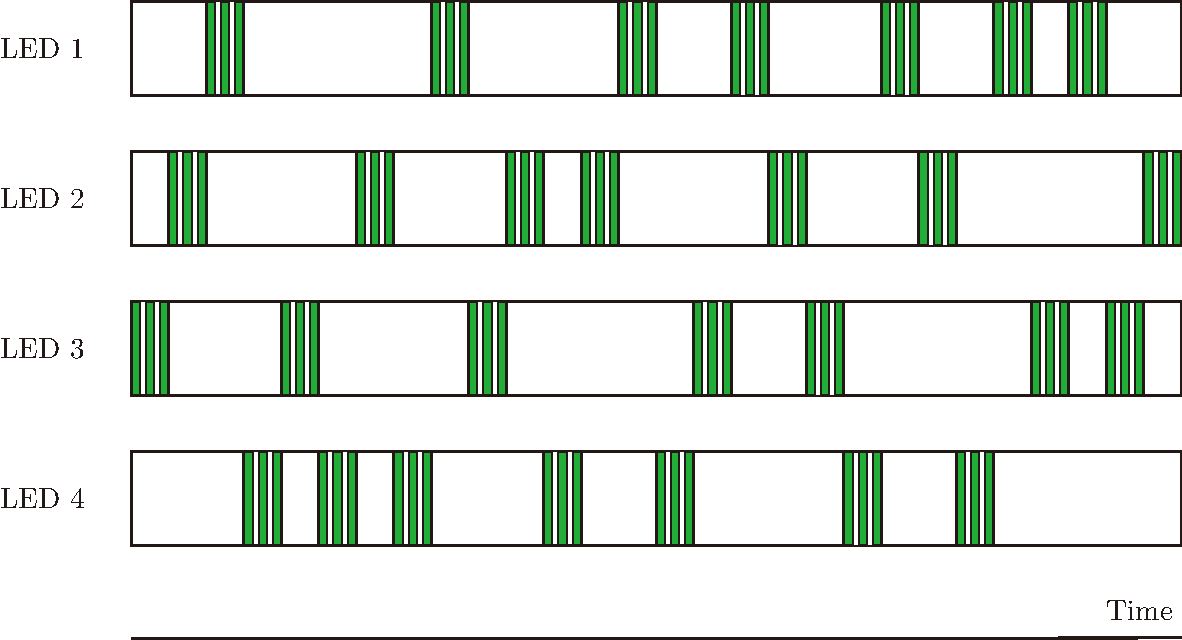
\includegraphics[scale = 0.65]{chapter7/mod_uni.pdf}
	\caption{Flickering type : Uniform random}
    \label{fig:mod_uni}
\end{figure}

\newpage
\subsection{Experiment result II}
\hspace{1.5cm} In this experiment, we use the method to find the accuracy be the same as the experiment I.
We obtain the raw EEG data from each subject and calculate the average data from the trials which be set.When we calculated the average of EEG data, we use this average data to find the accuracy of this experiment.

From the figure \ref{fig:comp2}, we have a comparison graph of the first experiment EXP A and the second experiment EXP B. Both are different in flickering types. EXP A's flickering type is regular, whereas EXP B has a uniform random type. This graph display the accuracy of EXP A and EXP B, where the trial = 9. The accuracy of EXP A is equal to 73.75\% and EXP B is equal to 85\%. We can see that EXP B is more accurate than EXP A in any trails that we use.

\begin{figure}[ht]
	\centering
	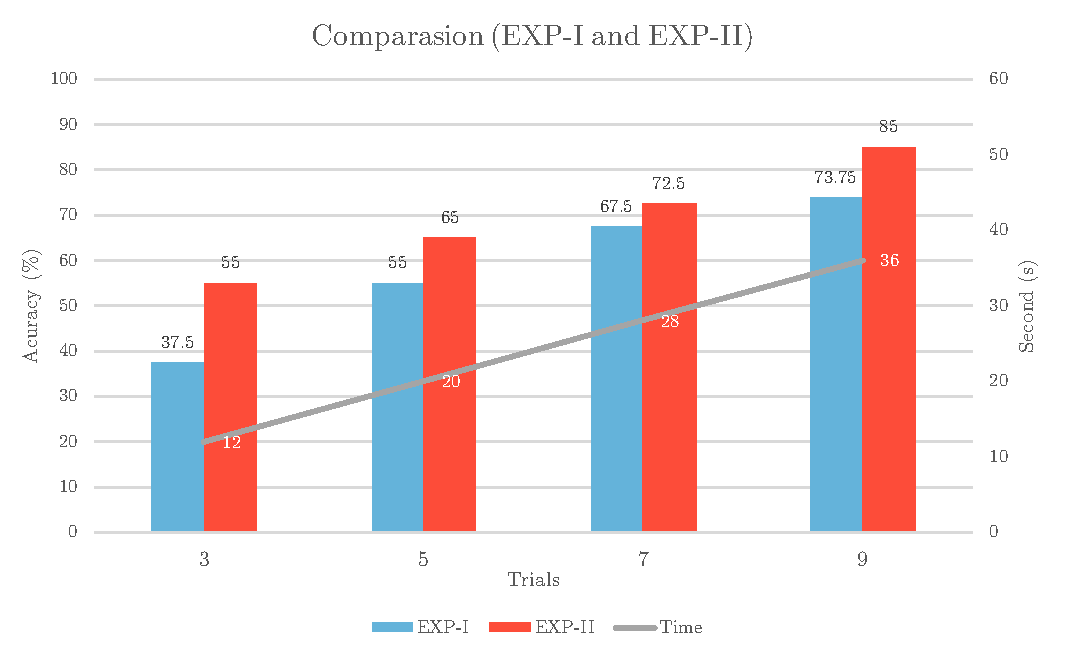
\includegraphics[scale = 0.8]{chapter7/result_12_2.pdf}
	\caption{Comparison between the result of experiment A and B}
    \label{fig:comp2}
\end{figure}

\begin{table}[ht]
\centering
\begin{tabular}{| c | c | c | c | c |}

			\hline 
			\multirow{2}{*}{\textbf{Trial}} & 
  			\multirow{2}{*}{\textbf{Total time [s]}}  & 
            \multirow{2}{*}{\textbf{Subject}} &
            \multicolumn{2}{c|}{\textbf{Accuracy of flickering type}} \\
            \cline{4-5}
            &&&\multicolumn{1}{c|}{\textbf{Regular}} &\multicolumn{1}{c|}{\textbf{Uniform}}  \\
			\hline 
			\multirow{4}{*}{3}&\multirow{4}{*}{11}&OK&40&50 \\
			\cline{3-5}
			&&WP&40&55 \\ \cline{3-5}
			&&SS&30&55 \\ \cline{3-5}
			&&NT&30&60 \\
            \hline
			\multirow{4}{*}{5}&\multirow{4}{*}{15}&OK&45&60 \\
			\cline{3-5}
			&&WP&55&70 \\ \cline{3-5}
			&&SS&65&65 \\ \cline{3-5}
			&&NT&55&75 \\
            \hline
            \multirow{4}{*}{7}&\multirow{4}{*}{19}&OK&65&70 \\
			\cline{3-5}
			&&WP&70&75 \\ \cline{3-5}
			&&SS&70&70 \\ \cline{3-5}
			&&NT&65&75 \\
            \hline 
            \multirow{4}{*}{9}&\multirow{4}{*}{23}&OK&70&85 \\
			\cline{3-5}
			&&WP&80&80 \\ \cline{3-5}
			&&SS&75&90 \\ \cline{3-5}
			&&NT&70&85 \\
            \hline 
		\end{tabular}       
\caption{Experiment result II}
\label{table:result2}
\end{table}

The result of this experiment is shown in Table \ref{table:result2} with same set of parameter for each stimulus, sample length, epoch time, duty cycle, intensity and frequency. First from the Table \ref{table:result2}, we compare between regular and uniform random. We can see the accuracy of "WP" in uniform random is better than regular of "WP" in the same row. The accuracy between regular and uniform random of "NT" in the last row of the table, regular is lower accuracy than uniform random. We found any subject have better accuracy in uniform random than regular of flickering type. We found another thing that is the trials of the experiment. The comparison of accuracy between "WP" in second row and "WP" in tenth row is the accuracy of "WP" in the tenth row is better than in the second row. The main factor is trial that we use in each experiment. We found that when we use more trials, the accuracy is increased same as experiment I.

\newpage
\section{Experiment III}
\subsection{Experimental Paradigm III}

\begin{itemize}
\item{\textbf{Subjects}}\newline
In this experiment, we use 4 subjects. There are SS,OK,WP and NT that is the nickname and firstname of subjects.

\begin{table}[ht]
\centering
\begin{tabular}{| P{.2\linewidth} | P{.2\linewidth} | P{.2\linewidth} |}
			\hline 
			\textbf{Subjects} & \textbf{Age}  & \textbf{Sex}\\
			\hline 
			SS & 22 & Male\\
			\hline 
			OK & 22 & Male\\
			\hline 
			WP & 21 & Male\\
			\hline 
			NT & 21 & Male\\
			\hline
		\end{tabular}       
\caption{Subjects of experiment III}
\label{table:2}
\end{table}

\item{\textbf{Visual Stimulator}}
In this experiment, we use 1 visual stimulator[LED 1($Y_1$)]
\item{\textbf{Stimulus}}
In this experiment, we separate the stimulus in 2 categories per one trial.
First, we obtain the EEG data of the subject to be baseline 6 seconds.
In active state, we obtain the EEG of the subject in 14 seconds.
\item{\textbf{Trials}}
We recorded 20 trials for each set of parameter.
\item{\textbf{Environment}}
In this experiment, we control the light illuminate value at 37 Lux.
\item{\textbf{Parameters}}\\
There are 4 parameters. First is frequency, duty cycle, light intensity, and light color.
\end{itemize}

\begin{table}[ht]
\centering
\begin{tabular}{| c | c | c | c |}
	\hline 
    \textbf{Frequency(Hz)}&\textbf{Duty}&\textbf{Intensity(\%)}&\textbf{color}\\
    \hline
    6&\multirow{24}{*}{\textbf{0.7}}&
    \multirow{24}{*}{50}&
    \multirow{24}{*}{Green}\\
    \cline{1-1}
    7&&&\\\cline{1-1}
    8&&&\\ \cline{1-1}
    9&&&\\ \cline{1-1}
    10&&&\\ \cline{1-1}
    11&&&\\ \cline{1-1}
    12&&&\\ \cline{1-1}
    13&&&\\\cline{1-1}
    14&&&\\ \cline{1-1}
    15&&&\\ \cline{1-1}
    16&&&\\ \cline{1-1}
    17&&&\\ \cline{1-1}
    18&&&\\ \cline{1-1}
    19&&&\\ \cline{1-1}
    20&&&\\ \cline{1-1}
    21&&&\\ \cline{1-1}
    22&&&\\ \cline{1-1}
    23&&&\\ \cline{1-1}
    24&&&\\ \cline{1-1}
    25&&&\\ \cline{1-1}
    26&&&\\ \cline{1-1}
    27&&&\\ \cline{1-1}
    28&&&\\ \cline{1-1}
    29&&&\\ 
    \hline
	\end{tabular}       
\caption{Experiment paradigm III}
\label{table:paradigm_3}
\end{table}

From table \ref{table:paradigm_3}, we set duty cycle = 0.7, light intensity 50\%, and light color = "Green". There are some differences in frequencies. We use frequencies from 6Hz to 29Hz and only 1 flicker in this experiment to obtain the EEG signal. The subjects observe the visual stimulator in for 20 trials each subject. Two channels position that we use in our experiment of visual cortex is $O_1$ and $O_2$. When EEG signal that we obtained is analyzed, we will calculate the accuracy of the experiment.

\newpage
\subsection{Experiment result III}
\hspace{1.5cm} We use this experiment to find the best accuracy among these frequencies to detect the fittest flicker to be used to control the program. We obtain the raw EEG data from each subject. In one trial, we use windowing function to separate the raw EEG data into segments. We use 512 samples for windowing function. When we get the windowing data. Then, the data will be analyzed by using the Fourier transform. Once the Fourier transform data is obtained, this data will be subtracted from the baseline. We will obtain other data to classify the flickers.The classification algorithm is peak detection. This algorithm is used to find the peak of the EEG data that is already classified, and will be used to calculate the accuracy of this experiment.

From the figure \ref{fig:avg_exp3}, This is the accuracy data of all subjects which are analyzed by the method mentioned in previous paragraph. The best accuracy is 83\% and belongs to the frequency at 15 Hz. The next accuracy is 81\$ and belongs to the frequency at 14 Hz. 

\begin{figure}[ht]
	\centering
	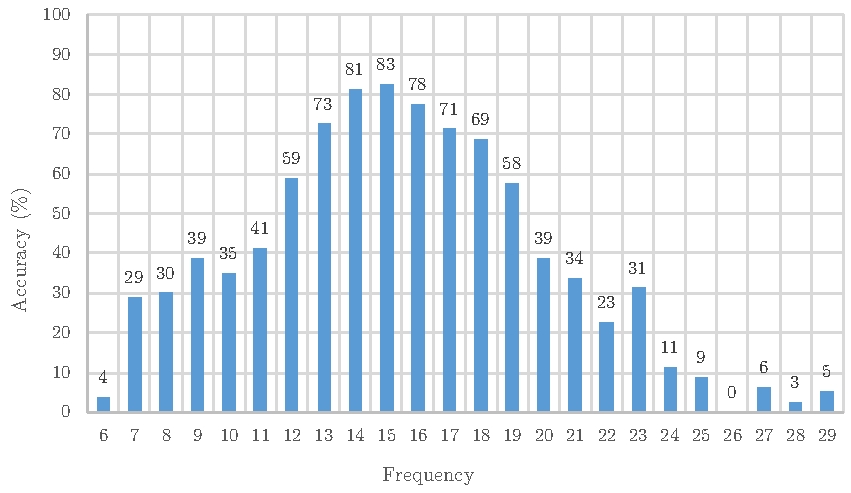
\includegraphics[scale = 1]{chapter7/exp4.pdf}
	\caption{The accuracy of all subjects}
    \label{fig:avg_exp3}
\end{figure}

\begin{table}[ht]
\centering
\begin{tabular}{| c | c | c | c |}

			\hline 
            \textbf{Frequency(Hz)}&\textbf{Subject}&\textbf{Accuracy(\%)}&\textbf{Averaged accuracy(\%)}\\
			\hline 
			\multirow{4}{*}{11}&OK&40&\multirow{4}{*}{41.25} \\
			\cline{2-3}
			&WP&35& \\ \cline{2-3}
			&SS&50& \\ \cline{2-3}
			&NT&40& \\
            \hline
			\multirow{4}{*}{12}&OK&65&\multirow{4}{*}{58.75} \\
			\cline{2-3}
			&WP&65& \\ \cline{2-3}
			&SS&60& \\ \cline{2-3}
			&NT&45& \\
            \hline
           \multirow{4}{*}{13}&OK&80&\multirow{4}{*}{72.5} \\
			\cline{2-3}
			&WP&80& \\ \cline{2-3}
			&SS&65& \\ \cline{2-3}
			&NT&65& \\
            \hline
            \multirow{4}{*}{14}&OK&80&\multirow{4}{*}{81.25} \\
			\cline{2-3}
			&WP&85& \\ \cline{2-3}
			&SS&90& \\ \cline{2-3}
			&NT&70& \\
            \hline
            \multirow{4}{*}{15}&OK&85&\multirow{4}{*}{82.5} \\
			\cline{2-3}
			&WP&85& \\ \cline{2-3}
			&SS&80& \\ \cline{2-3}
			&NT&80& \\
            \hline
            \multirow{4}{*}{16}&OK&80&\multirow{4}{*}{77.5} \\
			\cline{2-3}
			&WP&80& \\ \cline{2-3}
			&SS&75& \\ \cline{2-3}
			&NT&75& \\
            \hline
            \multirow{4}{*}{17}&OK&80&\multirow{4}{*}{71.25} \\
			\cline{2-3}
			&WP&70& \\ \cline{2-3}
			&SS&60& \\ \cline{2-3}
			&NT&75& \\
            \hline
    \end{tabular}
\caption{Experiment result III}
\label{table:result3}
\end{table}

\begin{table}[ht]
\centering
\begin{tabular}{| c | c | c | c |}   

            \hline 
            \textbf{Frequency(Hz)}&\textbf{Subject}&\textbf{Accuracy(\%)}&\textbf{Averaged accuracy(\%)}\\
            \hline
            \multirow{4}{*}{18}&OK&70&\multirow{4}{*}{68.75} \\
			\cline{2-3}
			&WP&65& \\ \cline{2-3}
			&SS&65& \\ \cline{2-3}
			&NT&75& \\
            \hline
            \multirow{4}{*}{19}&OK&60&\multirow{4}{*}{57.5} \\
			\cline{2-3}
			&WP&60& \\ \cline{2-3}
			&SS&55& \\ \cline{2-3}
			&NT&55& \\
            \hline
            \multirow{4}{*}{20}&OK&50&\multirow{4}{*}{38.75} \\
			\cline{2-3}
			&WP&35& \\ \cline{2-3}
			&SS&40& \\ \cline{2-3}
			&NT&30& \\
            \hline
            \multirow{4}{*}{21}&OK&45&\multirow{4}{*}{33.75} \\
			\cline{2-3}
			&WP&20& \\ \cline{2-3}
			&SS&30& \\ \cline{2-3}
			&NT&40& \\
            \hline
            \multirow{4}{*}{22}&OK&30&\multirow{4}{*}{22.5} \\
			\cline{2-3}
			&WP&25& \\ \cline{2-3}
			&SS&20& \\ \cline{2-3}
			&NT&15& \\
            \hline
            \multirow{4}{*}{23}&OK&30&\multirow{4}{*}{31.25} \\
			\cline{2-3}
			&WP&40& \\ \cline{2-3}
			&SS&35& \\ \cline{2-3}
			&NT&20& \\
            \hline
            \multirow{4}{*}{24}&OK&10&\multirow{4}{*}{11.25} \\
			\cline{2-3}
			&WP&15& \\ \cline{2-3}
			&SS&5& \\ \cline{2-3}
			&NT&15& \\
            \hline
            \multirow{4}{*}{25}&OK&10&\multirow{4}{*}{8.75} \\
			\cline{2-3}
			&WP&15& \\ \cline{2-3}
			&SS&5& \\ \cline{2-3}
			&NT&5& \\
            \hline
            \multirow{4}{*}{26}&OK&0&\multirow{4}{*}{0} \\
			\cline{2-3}
			&WP&0& \\ \cline{2-3}
			&SS&0& \\ \cline{2-3}
			&NT&0& \\
            \hline
            \multirow{4}{*}{27}&OK&5&\multirow{4}{*}{6.25} \\
			\cline{2-3}
			&WP&10& \\ \cline{2-3}
			&SS&5& \\ \cline{2-3}
			&NT&5& \\
            \hline
            \multirow{4}{*}{28}&OK&0&\multirow{4}{*}{2.5} \\
			\cline{2-3}
			&WP&0& \\ \cline{2-3}
			&SS&5& \\ \cline{2-3}
			&NT&5& \\
            \hline
            \multirow{4}{*}{29}&OK&5&\multirow{4}{*}{5} \\
			\cline{2-3}
			&WP&5& \\ \cline{2-3}
			&SS&5& \\ \cline{2-3}
			&NT&5& \\
            \hline
		\end{tabular}       
\caption{Experiment result III}
\label{table:result3_2}
\end{table}

From table \ref{table:result3} and table \ref{table:result3_2} shown the accuracy of all subject and average of accuracy of subjects in each frequency. There are 4 subjects in this experiment and each subject has difference accuracy. For example, subject "OK" in frequency 11 Hz has 40\% of accuracy and in frequency 13Hz has 80\%. Subject "WP" in frequency 11Hz has 35 accuracy rate and in frequency 13 Hz subject "WP" has 80\% of accuracy. We found that there are some range of frequency that subjects can respond in EEG signal.In this experiment, it is between frequency 13Hz to 18Hz that the accuracy is good to use.